\item \textbf{{[}HCI/PRELIM/9597/2014/P2/Q2{]} }
\begin{enumerate}
\item The Retail Company has engaged a software house to computerize its
operations. The project has been defined to contain the following
list of activities along with their required times for completion:
\noindent \begin{center}
\begin{tabular}{|c|l|c|c|}
\hline 
Activity & Description & Duration (Working Days) & Predecessor/s\tabularnewline
\hline 
\hline 
A & Requirement Analysis & 1 & \tabularnewline
\hline 
B & Systems Design & 3 & A\tabularnewline
\hline 
C & Programming & 5 & B\tabularnewline
\hline 
D & telecoms & 3 & B\tabularnewline
\hline 
E & Hardware Installation & 6 & B\tabularnewline
\hline 
F & Integration & 2 & C, D\tabularnewline
\hline 
G & System Testing & 2 & E, F\tabularnewline
\hline 
H & Training/Support & 1 & G\tabularnewline
\hline 
I & Handover and Go-Live & 1 & H\tabularnewline
\hline 
\end{tabular}
\par\end{center}
\begin{enumerate}
\item Complete the PERT chart below, indicating the earliest start time
and latest start time of each activity: 
\end{enumerate}
\begin{center}
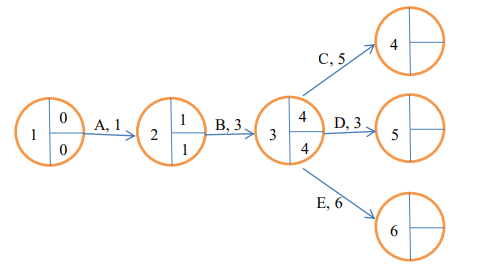
\includegraphics[width=0.65\paperwidth]{C:/Users/Admin/Desktop/Github/question_bank/LyX/static/img/9597-HCI-2014-P1-Q2}
\par\end{center}

\hfill{}{[}4{]}
\begin{enumerate}
\item State the critical path. \hfill{}{[}1{]}
\item State the elapsed time of the project. \hfill{}{[}1{]}
\item State 2 activities not on the critical path, as well as their slack
time. \hfill{}{[}2{]}
\end{enumerate}
\item The Gantt chart below is based on the above information. There are
three activities missing and three activities shown are incorrect.
Draw a sketch of the Gantt chart to show the correct version. 
\noindent \begin{center}
\begin{tabular}{c|c|c|c|c|c|c|c|c|c|c|c|c|c|c|c|c|c|c|c|}
\multicolumn{20}{c}{Weeks}\tabularnewline
\multicolumn{1}{c}{Activity} & \multicolumn{1}{c}{1} & \multicolumn{1}{c}{2} & \multicolumn{1}{c}{3} & \multicolumn{1}{c}{4} & \multicolumn{1}{c}{5} & \multicolumn{1}{c}{6} & \multicolumn{1}{c}{7} & \multicolumn{1}{c}{8} & \multicolumn{1}{c}{10} & \multicolumn{1}{c}{11} & \multicolumn{1}{c}{12} & \multicolumn{1}{c}{13} & \multicolumn{1}{c}{14} & \multicolumn{1}{c}{15} & \multicolumn{1}{c}{16} & \multicolumn{1}{c}{17} & \multicolumn{1}{c}{18} & \multicolumn{1}{c}{19} & \multicolumn{1}{c}{20}\tabularnewline
\cline{2-20} \cline{3-20} \cline{4-20} \cline{5-20} \cline{6-20} \cline{7-20} \cline{8-20} \cline{9-20} \cline{10-20} \cline{11-20} \cline{12-20} \cline{13-20} \cline{14-20} \cline{15-20} \cline{16-20} \cline{17-20} \cline{18-20} \cline{19-20} \cline{20-20} 
A & X &  &  &  &  &  &  &  &  &  &  &  &  &  &  &  &  &  & \tabularnewline
\cline{2-20} \cline{3-20} \cline{4-20} \cline{5-20} \cline{6-20} \cline{7-20} \cline{8-20} \cline{9-20} \cline{10-20} \cline{11-20} \cline{12-20} \cline{13-20} \cline{14-20} \cline{15-20} \cline{16-20} \cline{17-20} \cline{18-20} \cline{19-20} \cline{20-20} 
B &  & X & X & X &  &  &  &  &  &  &  &  &  &  &  &  &  &  & \tabularnewline
\cline{2-20} \cline{3-20} \cline{4-20} \cline{5-20} \cline{6-20} \cline{7-20} \cline{8-20} \cline{9-20} \cline{10-20} \cline{11-20} \cline{12-20} \cline{13-20} \cline{14-20} \cline{15-20} \cline{16-20} \cline{17-20} \cline{18-20} \cline{19-20} \cline{20-20} 
C &  &  &  &  &  & X & X & X & X & X &  &  &  &  &  &  &  &  & \tabularnewline
\cline{2-20} \cline{3-20} \cline{4-20} \cline{5-20} \cline{6-20} \cline{7-20} \cline{8-20} \cline{9-20} \cline{10-20} \cline{11-20} \cline{12-20} \cline{13-20} \cline{14-20} \cline{15-20} \cline{16-20} \cline{17-20} \cline{18-20} \cline{19-20} \cline{20-20} 
D &  &  &  &  &  &  &  & X & X & X &  &  &  &  &  &  &  &  & \tabularnewline
\cline{2-20} \cline{3-20} \cline{4-20} \cline{5-20} \cline{6-20} \cline{7-20} \cline{8-20} \cline{9-20} \cline{10-20} \cline{11-20} \cline{12-20} \cline{13-20} \cline{14-20} \cline{15-20} \cline{16-20} \cline{17-20} \cline{18-20} \cline{19-20} \cline{20-20} 
E &  &  &  &  & X & X & X & X & X & X &  &  &  &  &  &  &  &  & \tabularnewline
\cline{2-20} \cline{3-20} \cline{4-20} \cline{5-20} \cline{6-20} \cline{7-20} \cline{8-20} \cline{9-20} \cline{10-20} \cline{11-20} \cline{12-20} \cline{13-20} \cline{14-20} \cline{15-20} \cline{16-20} \cline{17-20} \cline{18-20} \cline{19-20} \cline{20-20} 
F &  &  &  &  &  &  &  &  &  &  & X & X &  &  &  &  &  &  & \tabularnewline
\cline{2-20} \cline{3-20} \cline{4-20} \cline{5-20} \cline{6-20} \cline{7-20} \cline{8-20} \cline{9-20} \cline{10-20} \cline{11-20} \cline{12-20} \cline{13-20} \cline{14-20} \cline{15-20} \cline{16-20} \cline{17-20} \cline{18-20} \cline{19-20} \cline{20-20} 
G &  &  &  &  &  &  &  &  &  &  &  &  &  &  &  &  &  &  & \tabularnewline
\cline{2-20} \cline{3-20} \cline{4-20} \cline{5-20} \cline{6-20} \cline{7-20} \cline{8-20} \cline{9-20} \cline{10-20} \cline{11-20} \cline{12-20} \cline{13-20} \cline{14-20} \cline{15-20} \cline{16-20} \cline{17-20} \cline{18-20} \cline{19-20} \cline{20-20} 
H &  &  &  &  &  &  &  &  &  &  &  &  &  &  &  &  &  &  & \tabularnewline
\cline{2-20} \cline{3-20} \cline{4-20} \cline{5-20} \cline{6-20} \cline{7-20} \cline{8-20} \cline{9-20} \cline{10-20} \cline{11-20} \cline{12-20} \cline{13-20} \cline{14-20} \cline{15-20} \cline{16-20} \cline{17-20} \cline{18-20} \cline{19-20} \cline{20-20} 
I &  &  &  &  &  &  &  &  &  &  &  &  &  &  &  &  &  &  & \tabularnewline
\cline{2-20} \cline{3-20} \cline{4-20} \cline{5-20} \cline{6-20} \cline{7-20} \cline{8-20} \cline{9-20} \cline{10-20} \cline{11-20} \cline{12-20} \cline{13-20} \cline{14-20} \cline{15-20} \cline{16-20} \cline{17-20} \cline{18-20} \cline{19-20} \cline{20-20} 
\end{tabular}
\par\end{center}

\end{enumerate}